\documentclass[ngerman, aspectratio=169]{beamer}

%packages
\usepackage[utf8]{inputenc}
\usepackage[english]{babel}
\usepackage{graphicx}
\usepackage{array}

\newcolumntype{L}[1]{>{\raggedright\let\newline\\\arraybackslash\hspace{0pt}}m{#1}}
\usepackage{ragged2e}

\usepackage{bm} % bold math
\usepackage{amsfonts}
\usepackage{amssymb}
\usepackage{mathtools}
\usepackage{amsmath}
\usepackage{multirow} % multi row in tables
\usepackage{scrextend}

\usepackage{tikz}

\usepackage{algorithmic}

%citations
\usepackage[style=verbose,backend=biber]{biblatex}
\addbibresource{references.bib}


%math font
\usefonttheme[onlymath]{serif}

%Beamer Template modifications
\definecolor{mainColor}{HTML}{0065A3} % HSR blue
\definecolor{invColor}{HTML}{28d79b} % OST pink
\definecolor{dgreen}{HTML}{38ad36} % Dark green

%\definecolor{mainColor}{HTML}{000000} % HSR blue
\setbeamercolor{palette primary}{bg=white,fg=mainColor}
\setbeamercolor{palette secondary}{bg=orange,fg=mainColor}
\setbeamercolor{palette tertiary}{bg=yellow,fg=red}
\setbeamercolor{palette quaternary}{bg=mainColor,fg=white} %bg = Top bar, fg = active top bar topic
\setbeamercolor{structure}{fg=black} % itemize, enumerate, etc (bullet points)
\setbeamercolor{section in toc}{fg=black} % TOC sections
\setbeamertemplate{section in toc}[sections numbered]
\setbeamertemplate{subsection in toc}{%
	\hspace{1.2em}{$\bullet$}~\inserttocsubsection\par}

\setbeamertemplate{itemize items}[circle]
\setbeamertemplate{description item}[circle]
\setbeamertemplate{title page}[default][colsep=-4bp,rounded=true]
\beamertemplatenavigationsymbolsempty

\setbeamercolor{footline}{fg=gray}
\setbeamertemplate{footline}{%
	\hfill\usebeamertemplate***{navigation symbols}
	\hspace{0.5cm}
	\insertframenumber{}\hspace{0.2cm}\vspace{0.2cm}
}

\usepackage{caption}
\captionsetup{labelformat=empty}

%Title Page
\title{Eigenwertperturbation}
\subtitle{Mathematisches Seminar 2020}
\author{Nicolas Tobler}
\institute{HSR Hochschule für Technik Rapperswil}

\date{25. Mai, 2020}

\DeclareMathOperator{\EX}{\mathbb{E}}% expected value
\DeclareMathOperator*{\argmax}{arg\,max}% argmax
%\DeclareMathOperator*{\max}{max}% max
\newcommand*{\QED}{\hfill\ensuremath{\blacksquare}}%

\newcommand*{\HL}{\textcolor{mainColor}}
\newcommand*{\RD}{\textcolor{red}}
\newcommand*{\BL}{\textcolor{blue}}
\newcommand*{\GN}{\textcolor{dgreen}}
\newcommand*{\GR}{\textcolor{lightgray}}

\newcommand\egeq{\stackrel{\mathclap{\normalfont\mbox{e.g.}}}{=}}

\usetikzlibrary{automata,arrows,positioning,calc}

\begin{document}
	
	\begin{frame}
		\titlepage
	\end{frame}
	
	\begin{frame}
		\frametitle{Content}
		\tableofcontents
	\end{frame}
	
	\section{Introduction}


	\begin{frame}
		\frametitle{Einleitung}

		\begin{block}{Eigenwertproblem}
			Gesucht sind Vektoren $v_i \in \mathbb {R}^{n} $, die durch $H$ nicht die Richtung ändern und sich nur mit $\lambda_i \in \mathbb R$ skalieren
			
            \begin{equation}
                \bm H \bm v_i = \lambda_i \bm v_i
			\end{equation}
        \end{block}

	\end{frame}

	\begin{frame}
		\frametitle{Berechnungsmethoden}

		\begin{itemize}
			\item Charakteristisches Polynom (Nur bis Ordnung 4)
			\item Jacobi-Verfahren
		\end{itemize}

		Verfahren sind sehr aufwendig und meist iterativ

	\end{frame}

	\begin{frame}
		\frametitle{Einleitung}
		
		

		\begin{block}{Machne Applikation benötigen nur Eigenwerte einer leicht veränderten Matrix $\bm H^{(1)}$, mit bekannten Eigenwerten}
			
			\begin{gather*}
				\bm H = \bm H_0 + \varepsilon \bm H_1 \\
				\varepsilon \in \mathbb{R^+} \ll 1 \\
				\lambda^{(0)}, \bm v^{(0)} \quad \text{bekannt}
			\end{gather*}

			Eigenvektoren von $H_0$ müssen zueinander othogonal sein
			\begin{itemize}
				\item Ist bei symetrischen Matrizen der Fall
			\end{itemize}
			

            $\rightarrow$ Eigenwertperturbation
        \end{block}

	\end{frame}

	\section{Anwendungen}

	\begin{frame}
        \frametitle{Anwendungen}

        \begin{block}{Erweiterung eines groben modells mit kleinen Einflüssen}
            \begin{itemize}
                \item Berechnen der Schrödingergleichung in Quantenmechanik %TODO check this
                \item Berechnung einer Trajektorie unter berücksichtigung der Luftfeuchtigkeit
                \item Einfluss von Planeten and die Umlaufbahn anderer Planeten
			\end{itemize}
        \end{block}

	\end{frame}


	\section{Herleitung}

	\begin{frame}
        \frametitle{Idee}

        \begin{block}{Nur linear teil einer Taylor approximation ist relevant}
            \begin{equation*}
				\bm H(\varepsilon) = \bm H_0 + \varepsilon \bm H_1 \GR{ + \varepsilon^2 \bm H_2  + \varepsilon^3 \bm H_3 + \dots}
			\end{equation*}

			\begin{align*}
				\bm v_i(\varepsilon) = \bm v_{0i} + \varepsilon \bm v_{1i} \GR{ + \varepsilon^2 \bm v_{2i}  + \varepsilon^3 \bm v_{3i} + \dots} \\
				\lambda_i(\varepsilon) = \lambda_{0i} + \varepsilon \lambda_{1i} \GR{ + \varepsilon^2 \lambda_{0i}  + \varepsilon^3 \lambda_{3i} + \dots}
			\end{align*}
        \end{block}

	\end{frame}

	\begin{frame}
        \frametitle{Herleitung}

        \begin{block}{Gesucht: Lösung von Gleichungssystem}

			\begin{align}
				\bm H(\varepsilon) \bm v_i(\varepsilon) &= \lambda_i(\varepsilon) \bm v_i(\varepsilon) \\
				(\bm H_0 + \varepsilon \bm H_1)
				(\bm v_{0i} + \varepsilon \bm v_{1i})
				&=
				(\lambda_{0i} + \varepsilon \lambda_{1i})
				(\bm v_{0i} + \varepsilon \bm v_{1i}) \\
				& \phantom{2} \vdots \nonumber\\
				\bm v_{0j}^T \bm H_0 \bm v_{0i}
				&=
				\delta_{ij} \lambda_{1i} + 
				( \lambda_{0i} - \lambda_{0j} )
				\bm v_{0j}^T  \bm v_{0i}
			\end{align}
			\begin{equation*}
				\delta_{ij} = \bm v_{0j}^T \bm H_0 \bm v_{0i}
				= \begin{cases}
					0 \quad (i \neq j),\\
					1 \quad (i = j)
					\end{cases}
			\end{equation*}
        \end{block}

	\end{frame}

	\begin{frame}
        \frametitle{Herleitung}

        \begin{block}{Gesucht: Lösung von Gleichungssystem}

			\begin{equation*}
				\bm v_{0j}^T \bm H_0 \bm v_{0i}
				=
				\delta_{ij} \lambda_{1i} + 
				( \lambda_{0i} - \lambda_{0j} )
				\bm v_{0j}^T  \bm v_{0i}
			\end{equation*}
			\begin{alignat*}{3}
				i = j \quad & \rightarrow  \quad && \lambda_{1i}&& = \bm v_{0i}^T \bm H_1 \bm v_{0i} \\
				i \neq j \quad & \rightarrow \quad && \bm v_{0j}^T \bm v_{1i}&& = \frac{\bm v_{0j}^T \bm H_1 \bm v_{0i}}{\lambda_{0i} - \lambda_{0j}}
			\end{alignat*}
        \end{block}
	\end{frame}

	\begin{frame}
        \frametitle{Herleitung}

        \begin{block}{Berechnung der Eigenwerte}

			\begin{alignat*}{3}
				i = j \quad & \rightarrow  \quad && \lambda_{1i}&& = \bm v_{0i}^T \bm H_1 \bm v_{0i} \\
				\GR{i \neq j \quad} & \GR{\rightarrow \quad} && \GR{\bm v_{0j}^T \bm v_{1i}} && \GR{= \frac{\bm v_{0j}^T \bm H_1 \bm v_{0i}}{\lambda_{0i} - \lambda_{0j}}}
			\end{alignat*}

			\begin{align*}
				\lambda_i(\varepsilon)
				&=
				\lambda_{0i} + \varepsilon \lambda_{1i} \\
				&=
				\lambda_{0i} + \varepsilon \bm v_{0i}^T \bm H_1 \bm v_{0i}
			\end{align*}
        \end{block}

	\end{frame}

	\begin{frame}
        \frametitle{Herleitung}

        \begin{block}{Berechnung der Eigenvektoren}
			\begin{columns}
				\begin{column}{0.5\textwidth}
					\begin{alignat*}{3}
						\GR{i = j \quad} & \GR{\rightarrow  \quad} && \GR{\lambda_{1i}} && \GR{= \bm v_{0i}^T \bm H_1 \bm v_{0i}} \\
						i \neq j \quad & \rightarrow \quad && \bm v_{0j}^T \bm v_{1i}&& = \frac{\bm v_{0j}^T \bm H_1 \bm v_{0i}}{\lambda_{0i} - \lambda_{0j}}
					\end{alignat*}
					\begin{align*}
						\bm v_i(\varepsilon)
						&=
						\bm v_{0i} + \varepsilon \bm v_{1i} \\
						&=
						\bm v_{0i} + \varepsilon \sum_{j} ( \bm v_{0j}^T \bm v_{1i}) \, \bm v_{0j} \\
						&=
						\bm v_{0i} + \varepsilon ( \bm v_{0i}^T \bm v_{1i}) \bm v_{0i} + \varepsilon \sum_{j \neq i} (\bm v_{0j}^T v_{1i}) \, \bm v_{0j}
					\end{align*}
				\end{column}
				\begin{column}{0.4\textwidth}
					\begin{center}
						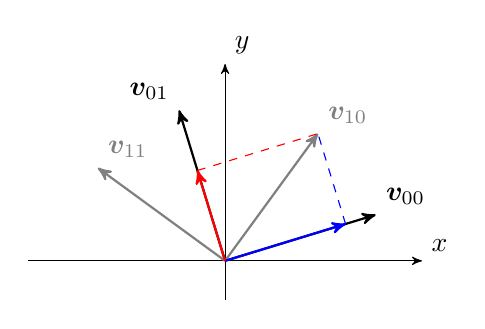
\begin{tikzpicture}[->, >=stealth', auto, node distance=2cm]

    \draw[] (0,-0.5) -- (0,2.5) node[above right]{$y$} ;
    \draw[]  (-2.5,0) -- (2.5, 0) node[above right]{$x$} ;

    \begin{scope}[rotate=17]
        \draw[thick] (0,0) -- (2,0) node[above right]{$\bm v_{00}$} ;
        \draw[thick] (0,0) -- (0,2) node[above left]{$\bm v_{01}$} ;

        \draw[thick, gray] (0,0) -- (1.6,1.2) node[above right]{$\bm v_{10}$} ;
        \draw[thick, gray] (0,0) -- (-1.2,1.6) node[above right]{$\bm v_{11}$} ;

        \draw[blue, dashed, -] (1.6,0) -- (1.6,1.2) ;
        \draw[red, dashed, -] (0,1.2) -- (1.6,1.2) ;

        \draw[thick, blue] (0,0) -- (1.6,0) ;
        \draw[thick, red] (0,0) -- (0,1.2) ;

    \end{scope}

\end{tikzpicture}
					\end{center}
				\end{column}
			\end{columns}
        \end{block}
	\end{frame}

	\begin{frame}
        \frametitle{Herleitung}

		\begin{block}{Berechnung der Eigenvektoren}
			\begin{alignat*}{3}
				\GR{i = j \quad} & \GR{\rightarrow  \quad} && \GR{\lambda_{1i}} && \GR{= \bm v_{0i}^T \bm H_1 \bm v_{0i}} \\
				i \neq j \quad & \rightarrow \quad && \bm v_{0j}^T \bm v_{1i}&& = \frac{\bm v_{0j}^T \bm H_1 \bm v_{0i}}{\lambda_{0i} - \lambda_{0j}}
			\end{alignat*}
			\begin{align*}
				\bm v_i(\varepsilon)
				&=
				\bm v_{0i} + \varepsilon ( \bm v_{0i}^T \bm v_{1i}) \bm v_{0i} + \varepsilon \sum_{j \neq i} (\bm v_{0j}^T \bm v_{1i}) \, \bm v_{0j} \\
				&=
				\bm v_{0i} ( 1 + (\bm v_{0i}^T \bm v_{1i}) ) + \varepsilon \sum_{j \neq i}
				\frac{\bm v_{0j}^T \bm H_1 \bm v_{0i}}{\lambda_{0i} - \lambda_{0j}}
				\, \bm v_{0j} \\
				&=
				\bm v_{0i} ( 1 + \mathrm{Im}(\varepsilon \gamma) ) + \varepsilon \sum_{j \neq i}
				\frac{\bm v_{0j}^T \bm H_1 \bm v_{0i}}{\lambda_{0i} - \lambda_{0j}}
				\, \bm v_{0j}
				\quad
				\QED
			\end{align*}
        \end{block}
	\end{frame}

	\begin{frame}
        \frametitle{Herleitung}

		\begin{block}{Zusammenfassung}
			\begin{align*}
				\lambda_i(\varepsilon)
				&=
				\lambda_{0i} + \varepsilon \bm v_{0i}^T \bm H_1 \bm v_{0i}\\
				\bm v_i(\varepsilon)
				&=
				\lambda_{0i} + \varepsilon \bm v_{0i}^T \bm H_1 \bm v_{0i}
				\bm v_{0i} ( 1 + \mathrm{Im}(\varepsilon \gamma) ) + \varepsilon \sum_{j \neq i}
				\frac{\bm v_{0j}^T \bm H_1 \bm v_{0i}}{\lambda_{0i} - \lambda_{0j}}
				\, \bm v_{0j}
			\end{align*}
        \end{block}
	\end{frame}

	\begin{frame}
        \frametitle{Beispiel 2D}
			\begin{columns}
				\begin{column}{0.4\textwidth}
					\begin{equation*}
						\BL{\bm H(\varepsilon)} = \GR{\bm H_0} + \GN{\varepsilon \bm H_1}
					\end{equation*}
					\begin{align*}
						\text{Korrekt} :& \quad  \BL{\bm v(\varepsilon)} \\
						\text{Perturbiert} :& \quad  \RD{\bm v(\varepsilon)}
					\end{align*}
				\end{column}
				\begin{column}{0.59\textwidth}
					\begin{center}
						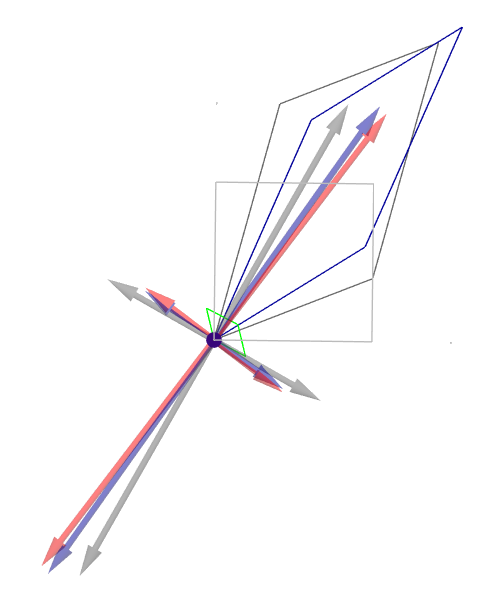
\includegraphics[scale=0.40]{img/bsp2d.png}
					\end{center}
				\end{column}
			\end{columns}
	\end{frame}

	\begin{frame}
        \frametitle{Beispiel 3D}
			\begin{columns}
				\begin{column}{0.4\textwidth}
					\begin{equation*}
						\BL{\bm H(\varepsilon)} = \GR{\bm H_0} + \GN{\varepsilon \bm H_1}
					\end{equation*}
					\begin{align*}
						\text{Korrekt} :& \quad  \BL{\bm v(\varepsilon)} \\
						\text{Perturbiert} :& \quad  \RD{\bm v(\varepsilon)}
					\end{align*}
				\end{column}
				\begin{column}{0.59\textwidth}
					\begin{center}
						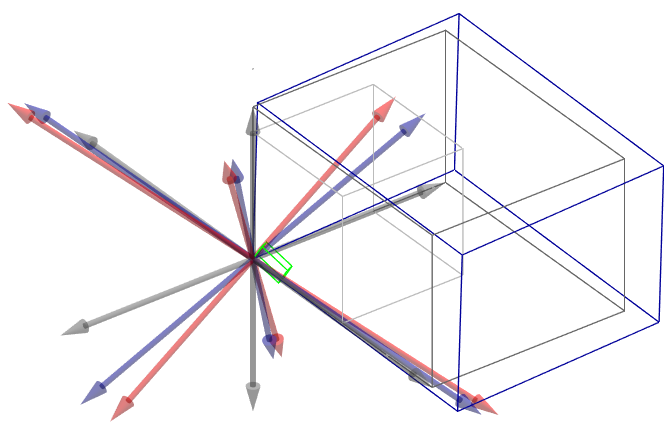
\includegraphics[scale=0.40]{img/bsp3d.png}
					\end{center}
				\end{column}
			\end{columns}
	\end{frame}

	\section{Entartung}

	\begin{frame}
        \frametitle{Entartung}

		\begin{block}{Was, wenn zwei oder mehr Eigenwerte gleich sind?}

			\begin{columns}
				\begin{column}{0.59\textwidth}

					\begin{center}
						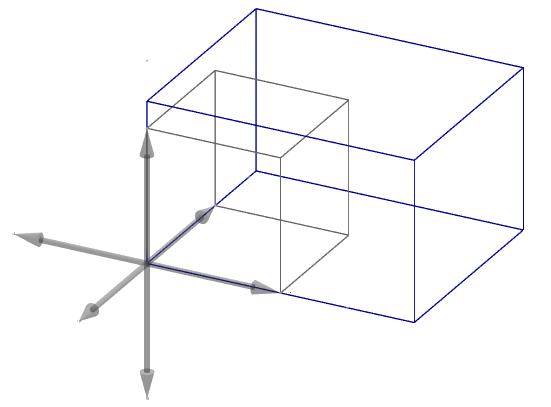
\includegraphics[scale=0.3]{img/eigenvectors.png}
					\end{center}
					\begin{equation*}
						\bm H_0 = 
						\begin{pmatrix}
							2 & 0 & 0\\
							0 & 1.6 & 0\\
							0 & 0 & 1.2
						\end{pmatrix}
					\end{equation*}
				\end{column}
				\begin{column}{0.40\textwidth}
					\begin{center}
						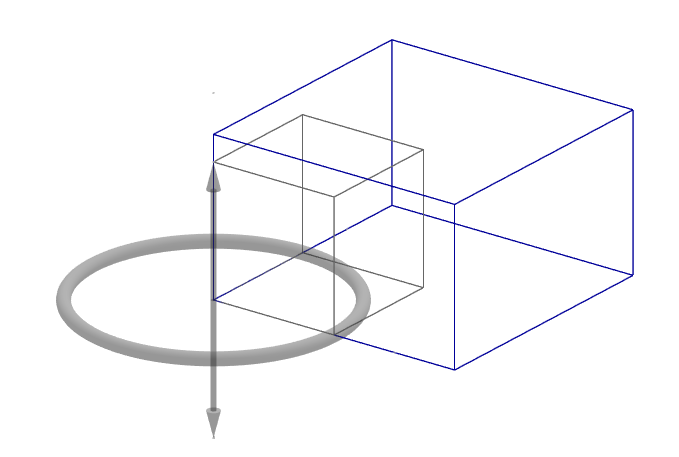
\includegraphics[scale=0.3]{img/entartung.png}
					\end{center}
					\begin{equation*}
						\bm H_0 = 
						\begin{pmatrix}
							2 & 0 & 0\\
							0 & 2 & 0\\
							0 & 0 & 1.2
						\end{pmatrix}
					\end{equation*}
				\end{column}
			\end{columns}
		\end{block}
	\end{frame}

	\begin{frame}
        \frametitle{Entartung}

		\begin{block}{Was, wenn zwei oder mehr Eigenwerte gleich sind?}

			\begin{equation*}
				\bm H_0 = 
				\begin{pmatrix}
					2 & 0 & 0\\
					0 & 2 & 0\\
					0 & 0 & 1.2
				\end{pmatrix}
			\end{equation*}
			\begin{equation*}
				\lambda_0 = 
				\{
					2, 2, 1.2
				\}
				\quad
				\bm v_0 = 
				\begin{pmatrix}
					? & ? & 0\\
					? & ? & 0\\
					0 & 0 & 1.2
				\end{pmatrix}
			\end{equation*}
			Die Eigenvektoren sind nicht mehr eindeutig.

			Sie werden von numerischen Programmen einfach gewählt:
			\begin{equation*}
				\text{z.B.}
				\quad
				\begin{pmatrix}
					2 & 0 & 0\\
					0 & 2 & 0\\
					0 & 0 & 1.2
				\end{pmatrix}
				\quad
				\text{oder}
				\quad
				\begin{pmatrix}
					1.2 & 1.6 & 0\\
					-1.6 & 1.2 & 0\\
					 0 & 0 & 1.2
				\end{pmatrix}
			\end{equation*}
		\end{block}
	\end{frame}

	\begin{frame}
        \frametitle{Entartung}

		\begin{block}{Entartete Eigenwerte können Division durch Null auslösen}

			\begin{equation*}
				\bm v_i(\varepsilon)
				=
				\bm v_{0i} ( 1+ \mathrm{Im}(\varepsilon \gamma)) + \varepsilon \sum_{j \neq i}
				\frac{\GN{\bm v_{0j}^T \bm H_1 \bm v_{0i}}}{\RD{\lambda_{0i} - \lambda_{0j}}}
				\, \bm v_{0j}
			\end{equation*}
		\end{block}
		\begin{block}{Idee:}
			Kein Problem, wenn Zähler auch Null ist

			Falls entartet, wähle $\bm v_{0i}$, so dass
			\begin{equation*}
				\GN{\bm v_{0j}^T \bm H_1 \bm v_{0i}} = 0 \quad \forall \quad i,j \quad entartet
			\end{equation*}
		\end{block}
	\end{frame}


	\begin{frame}
        \frametitle{Entartung}

		\begin{columns}
			\begin{column}{0.59\textwidth}

				Bilde $\bm H_1$ auf basis von entarteten, zufällig gewählten Eigenvektoren ab
				\begin{equation*}
					\bm H^\prime = \bm v_{0i}^T \bm H_1 \bm v_{0i} \quad \forall \quad i \quad entartet
				\end{equation*}
				Löse kleines Eigenwertproblem (alle $\lambda_i$ sind noch bekannt)
				\begin{equation*}
					\bm H^\prime \bm v_{i}^\prime = \lambda_{i} \bm v_i^\prime \quad \forall \quad i \quad entartet
				\end{equation*}
				Transformiere gefundene Eigenvektoren zurück und verwende diese als die neuen, korrekten Eigenvektoren
				\begin{equation*}
					\bm v_{0i} \gets \bm v_{0i} \bm v_{i}^\prime  \quad \forall \quad i \quad entartet
				\end{equation*}
			\end{column}
			\begin{column}{0.40\textwidth}
				\begin{center}
					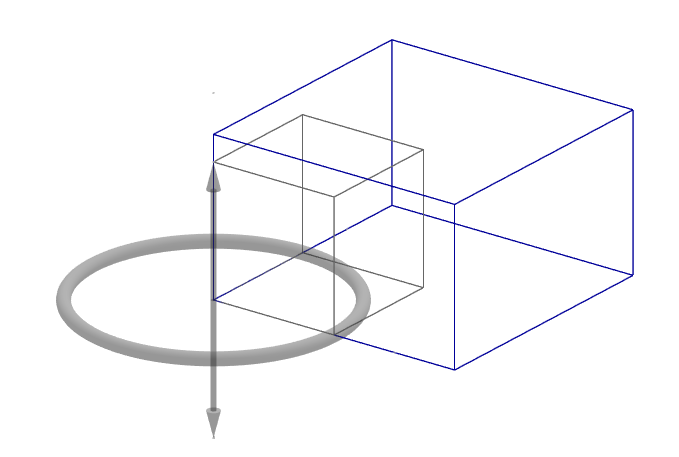
\includegraphics[scale=0.25]{img/entartung.png}
				\end{center}
				\begin{equation*}
					\vdots
				\end{equation*}
				\begin{center}
					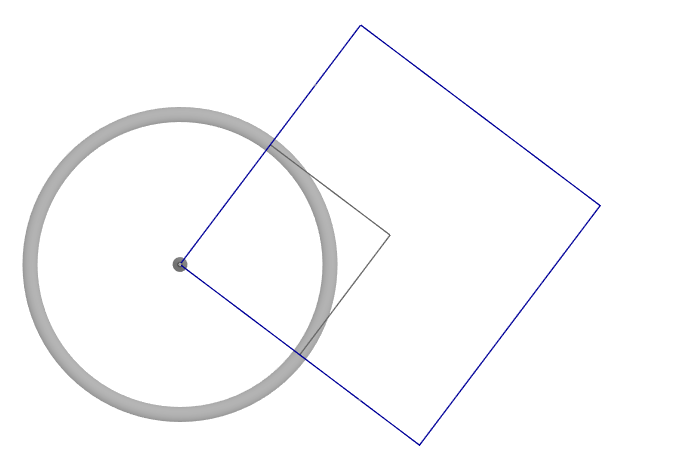
\includegraphics[scale=0.25]{img/entartung2.png}
				\end{center}
			\end{column}
		\end{columns}
	\end{frame}

	\begin{frame}
        \frametitle{Entartung}

		\begin{align*}
			\lambda_i(\varepsilon)
			& \gets
			\lambda_{0i} + \varepsilon \bm v_{0i}^T \bm H_1 \bm v_{0i}\\
			\bm H^\prime & \gets \bm v_{0i}^T \bm H_1 \bm v_{0i} \quad \forall \quad i \quad entartet \\
			\bm v^\prime & \gets \mathrm{Eig} \Big( \bm H^\prime \Big) \\
			\bm v_{0i} & \gets \bm v_{0i} \bm v^\prime  \quad \forall \quad i \quad entartet \\
			\bm v_i(\varepsilon)
			& \gets
			\lambda_{0i} + \varepsilon \bm v_{0i}^T \bm H_1 \bm v_{0i}
				\bm v_{0i} ( 1 + \mathrm{Im}(\varepsilon \gamma) ) + \varepsilon \sum_{j \neq i, \,nicht\,entartet}
				\frac{\bm v_{0j}^T \bm H_1 \bm v_{0i}}{\lambda_{0i} - \lambda_{0j}}
				\, \bm v_{0j}
		\end{align*}
		
	\end{frame}

	\begin{frame}
        \frametitle{Entartung}
		\begin{block}{Anwendung}
			Aufspaltung der Energieniveaus von Atomen in der Quantenmechanik
			\begin{center}
				\includegraphics[scale=0.25, clip, trim=0 85 0 0]{img/WasserstoffAufspaltung.pdf}
				\footnote{Quantenmechanik, Mathematisches Seminar, Andreas Müller et. al (CC0 1.0)}
			\end{center}
		\end{block}
	\end{frame}

\end{document}
